\documentclass{article}
\usepackage{tikz}
\usetikzlibrary{patterns}

\begin{document}

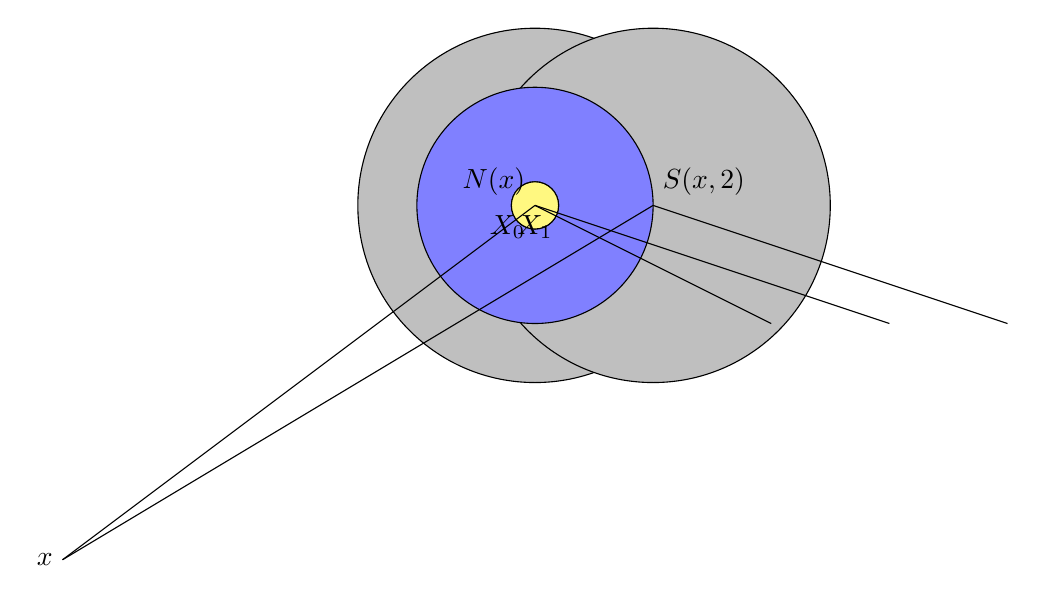
\begin{tikzpicture}[scale=1.5]

% Define coordinates
\coordinate (x) at (-1, -1);
\coordinate (y) at (3, 2);
\coordinate (z) at (4, 2);
\coordinate (a) at (5, 1);
\coordinate (b) at (6, 1);
\coordinate (c) at (7, 1);

% Draw circles
\draw[fill=gray!50] (y) circle (1.5);
\draw[fill=gray!50] (z) circle (1.5);
\draw[fill=blue!50] (y) circle (1);
\draw[fill=red!50] (y) circle (0.2);
\draw[fill=yellow!50] (y) circle (0.2);

% Draw lines
\draw (x) -- (y);
\draw (x) -- (z);
\draw (y) -- (a);
\draw (y) -- (b);
\draw (z) -- (c);

% Label points
\node at (x) [left] {$x$};
\node at (y) [above left] {$N(x)$};
\node at (z) [above right] {$S(x, 2)$};
\node at (a) [right] {};
\node at (b) [right] {};
\node at (c) [right] {};

% Label sets
\node at (y) [below left] {$X_0$};
\node at (y) [below] {$X_1$};

\end{tikzpicture}

\end{document}